\documentclass{article}

%Packages
\usepackage{graphicx}
\usepackage{grffile}
\usepackage{float}

%Margins
\usepackage[
	margin=2cm,
	includefoot
	]{geometry}

%Images
\usepackage{graphicx}

\graphicspath{{images/}}

%Headers and Footers
\usepackage{fancyhdr}
\pagestyle{fancy}
\fancyhead{}
\fancyfoot{}
\fancyfoot[R]{\thepage}
\renewcommand{\headrulewidth}{0pt}
\renewcommand{\footrulewidth}{0pt}


%Details
\title{
Software Requirements Specification and 
Technology Neutral Process Design
(University of Pretoria - Postgraduate Paper Interaction Portal)
}
\date{2016-02-15}
\author{Team Juliet}

%Document start
\begin{document}

%Title Page
\begin{titlepage}
	\begin{center}
		
\includegraphics[width=10cm]{UP.jpg}  \\
		[1cm]
		\line(1,0){300} \\
		[0.4cm]
		\textsc{\huge
			Software Requirements Specification and 
			Technology Neutral Process Design
			(University of Pretoria - Postgraduate Paper Interaction Portal)
		} \\
		[0.1cm]
		\line(1,0){300} \\
		[0.4cm]
		\textsc{\Large
			Team Juliet
		} \\

	\end{center}
	\begin{flushright}
	\textsc{\Large
	Quinton Weenink\\ 
	u13176545\\
	Vuyani Shabangu\\
	u11171139\\
	Ruan Klinkert\\
	u14022282\\
	Reinhardt Cromhout\\
	u14009936\\
	Rohan Chhipa\\
	u14188377\\
	Brandon Wardley\\
	u29005150\\
	}
	\end{flushright}
\end{titlepage}

%Table of contents
\tableofcontents
\thispagestyle{empty}
\cleardoublepage

%Content
\setcounter{page}{1}
\section{Introduction}
%\lable{sec:intro} for some readon i cant get the lables to work maybe you guys will have some luck
The purpose of this document is to describe the requirements of the “Postgraduate Paper Interaction Portal” application, by illustrating the purpose and uses of the system, as well as the development of the system. The system constraints, interface and various interactions will also be discussed, and testable quality requirements will be provided where applicable.

\section{Vision}
	The project aims to equip people who see a need for a drone. Without having to own a very expensive drone or have the expertise to operate the drone which can be as expensive to acquire. With the Drone Mission Project in full effect customers can achieve maximum output out of every mission while the business continues to reap in the rewards of the service portal we provide.

\section{Background}
	The Drone Mission project is aimed at equipping a client that would need the services of the drone but does not own a drone or the expertise to control the drone. The client or user would register to the website service and request the details of his mission such as time, place and if it is a recurring mission every hour, day, week, etc. The system would process all details and a drone operator will send information back to system to fly the drone. Information is captured and sent to the client efficiently.

\section{Functional requirements and application design}
%\lable{sec:funcreq}
We will now speak on the different subsystems and show the use cases, service contracts, required functionality and process specifications. Our subsetions that we will focus on is the operator, mission and the user as these are the main subsections that make our project.

\subsection{Operator subsystem}
	\subsubsection{Use cases}

		\begin{flushleft}
			\textbf{Critical}
				\begin{itemize}
	  				\item Add drone
	  				\item Remove drone
					\item Assign research group leader
					\item View research group unit score
				\end{itemize}

			\textbf{Nice-To-Have}
				\begin{itemize}
	  				\item Edit drone
				\end{itemize}
		\end{flushleft}

	\subsubsection{Services Contracts}

		\begin{figure}[H]
			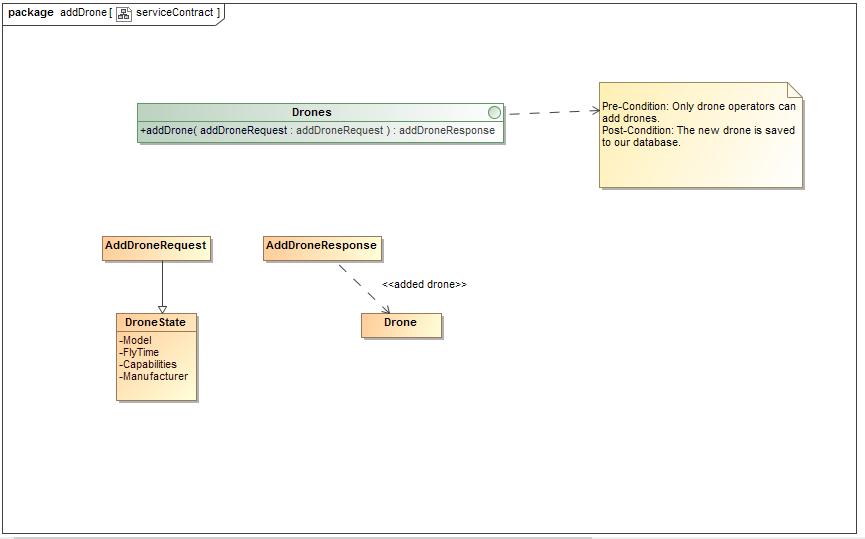
\includegraphics[width=\textwidth]{SC_add.png}  \\
			\caption{Services Contract : addDrone}
		\end{figure}
		\begin{figure}[H]
			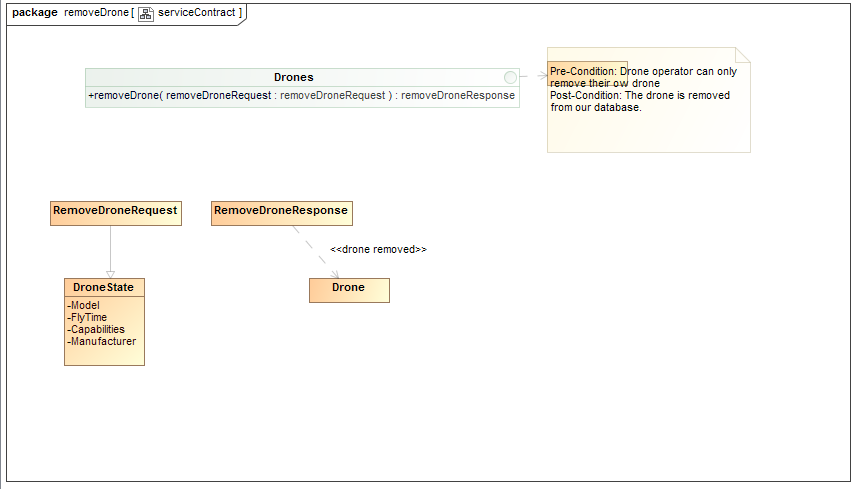
\includegraphics[width=\textwidth]{sc_delete.png}  \\
			\caption{Services Contract : removeDrone}
		\end{figure}
		\begin{figure}[H]
			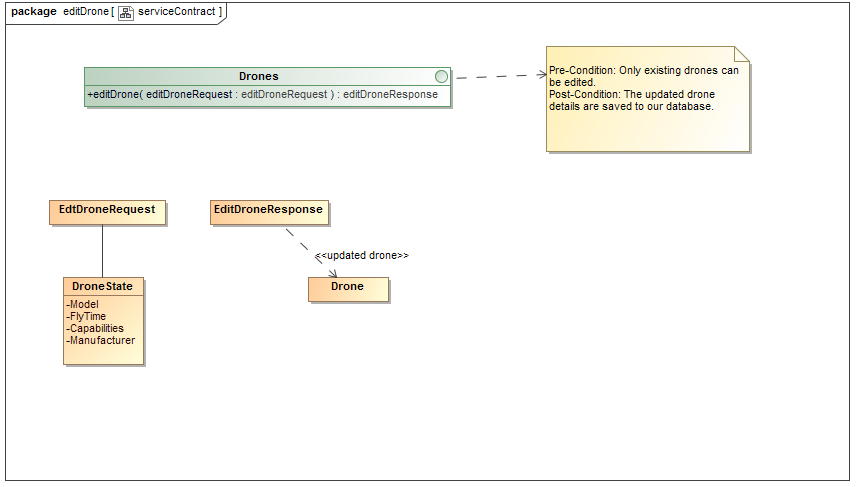
\includegraphics[width=\textwidth]{sc_edit.png}  \\
			\caption{Services Contract : editDrone}
		\end{figure}

	\subsubsection{Required functionality}
	
		\begin{figure}[H]
			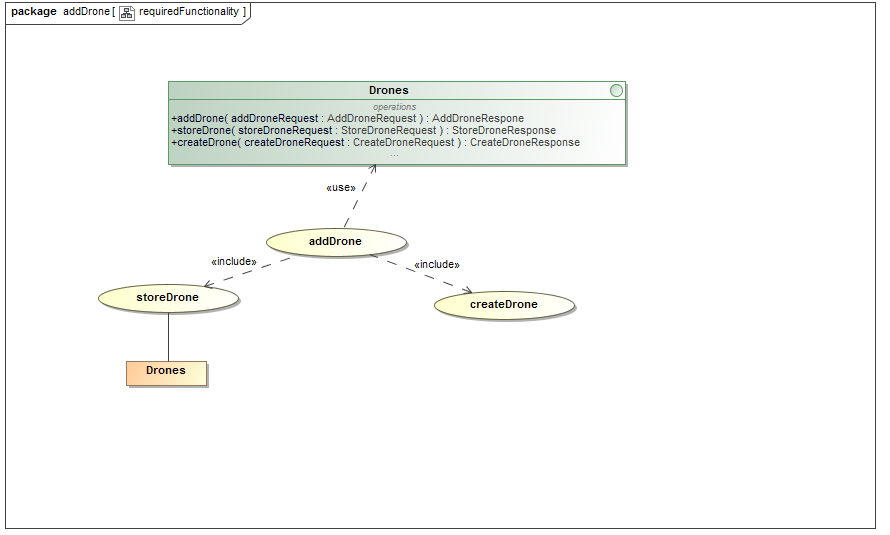
\includegraphics[width=\textwidth]{rf_add.png}  \\
			\caption{Functional Requirements : addDrone}
		\end{figure}
		\begin{figure}[H]
			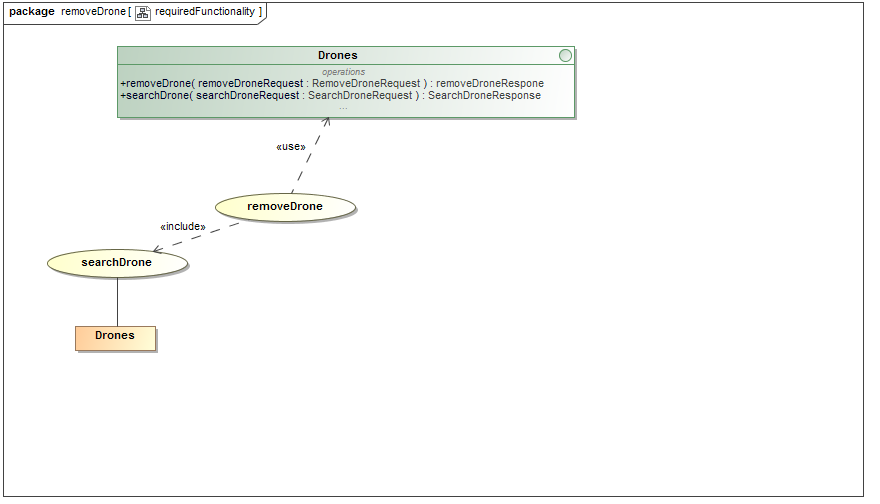
\includegraphics[width=\textwidth]{rf_remove.png}  \\
			\caption{Functional Requirements : removeDrone}
		\end{figure}
		\begin{figure}[H]
			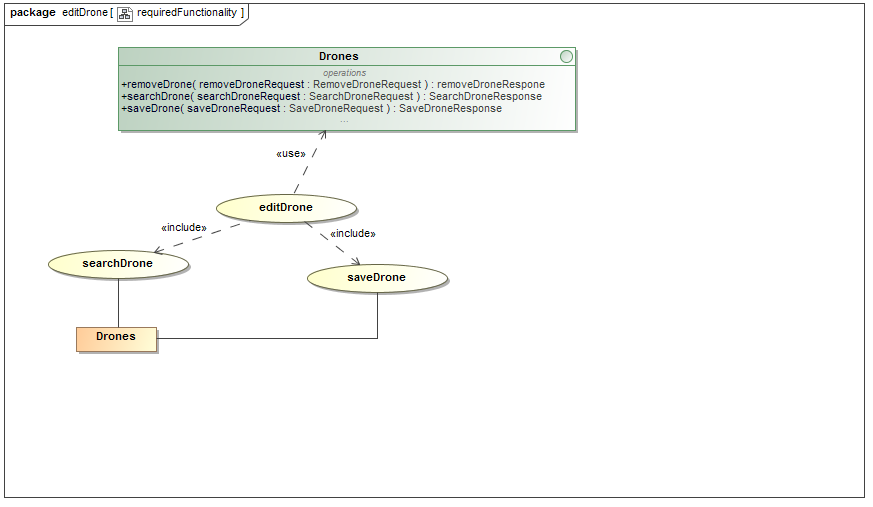
\includegraphics[width=\textwidth]{rf.png}  \\
			\caption{Functional Requirements : editDrone}
		\end{figure}
	

	\subsubsection{Process specifications}
	
		\begin{figure}[H]
			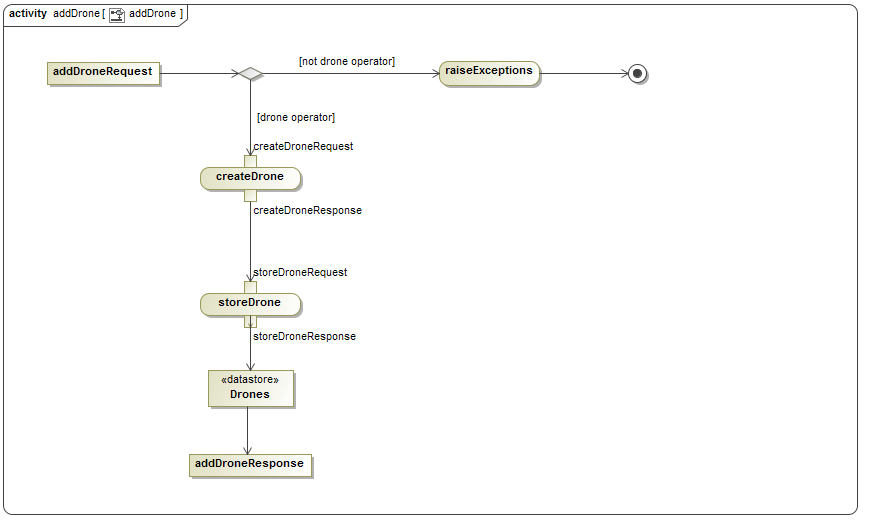
\includegraphics[width=\textwidth]{ps_add.png}  \\
			\caption{Process Specification : addDrone}
		\end{figure}
		\begin{figure}[H]
			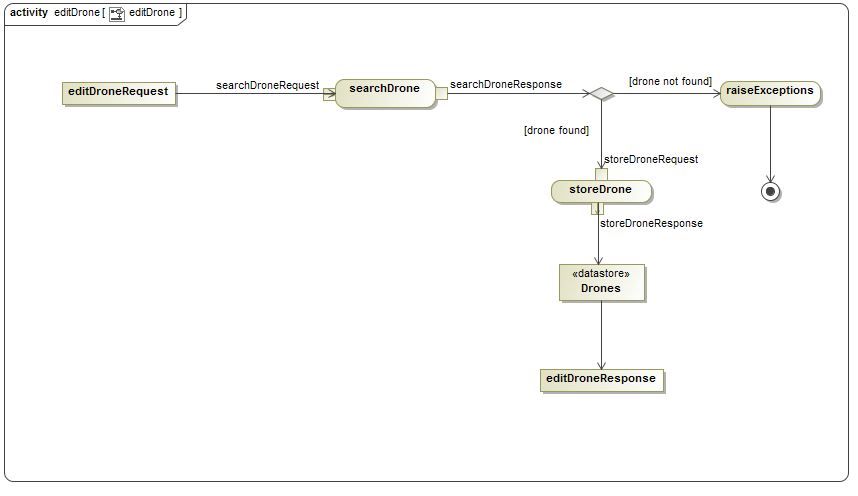
\includegraphics[width=\textwidth]{ps_edit.png}  \\
			\caption{Process Specification : editDrone}
		\end{figure}
		\begin{figure}[H]
			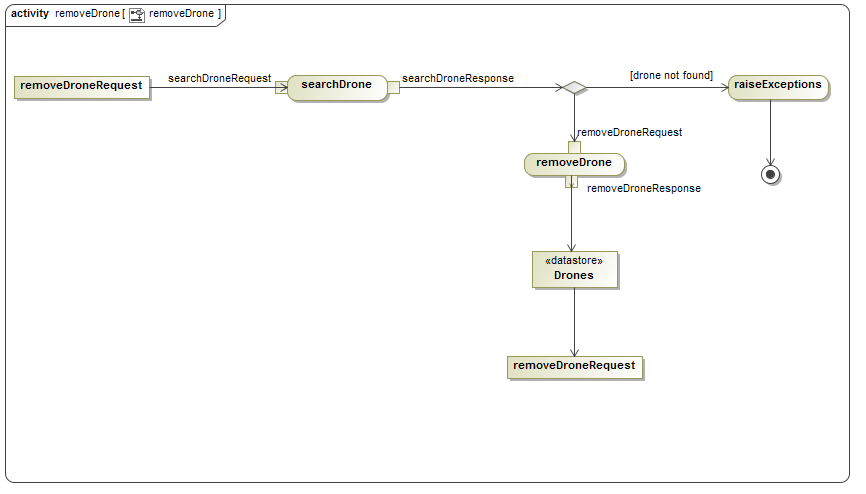
\includegraphics[width=\textwidth]{ps_delete.png}  \\
			\caption{Process Specification : removeDrone}
		\end{figure}
		%To include diagrams for process specifications here.
		
	
	
\newpage

	\subsection{Domain Model}
	
	The domain model shows the data structure requirements of the Researcher Support System, as well as the relationships between the different domain objects. 

	\begin{figure}[H]
		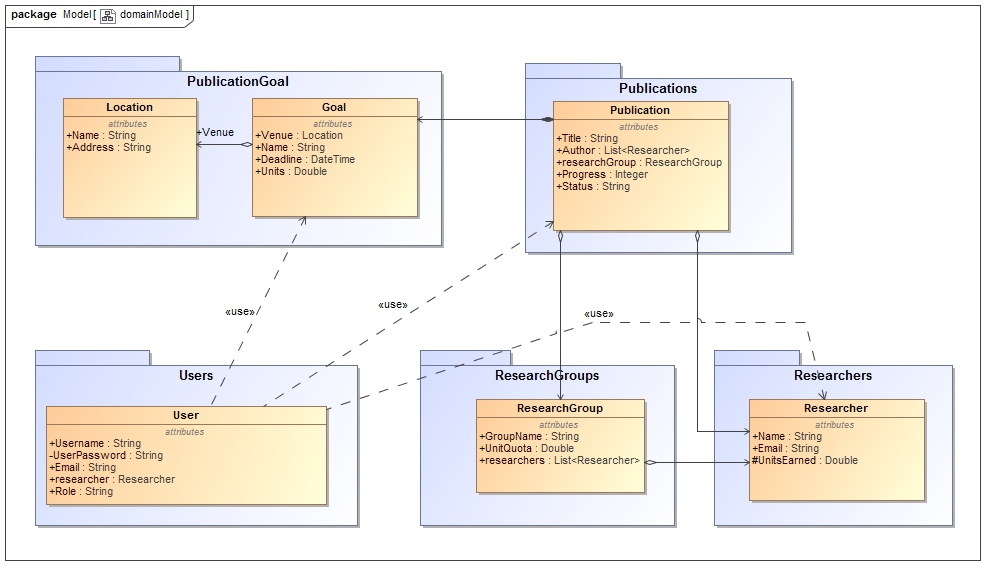
\includegraphics[width=\textwidth]{domainModelB.jpg}  \\
		\caption{Domain Model}
	\end{figure}
	
\newpage

\section{Mission subsection}
%\lable{sec:open}
\subsubsection{Use cases}

		\begin{flushleft}
			\textbf{Critical}
				\begin{itemize}
	  				\item Add mission
	  				\item Delete mission
	  				\item View mission
				\end{itemize}
				
				\begin{figure}[H]
					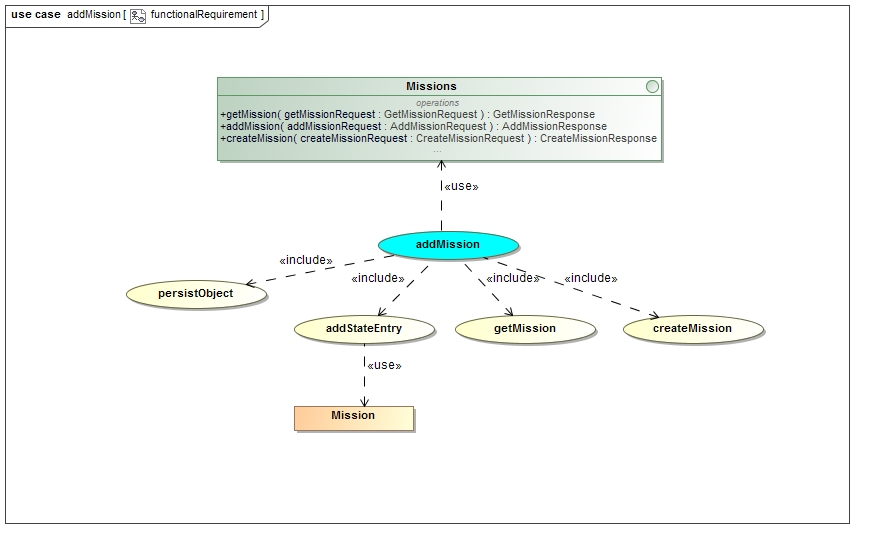
\includegraphics[width=\textwidth]{functionalRequirement_addmission.jpg}  \\
					\caption{Use case : addMission}
				\end{figure}
				
				\begin{figure}[H]
					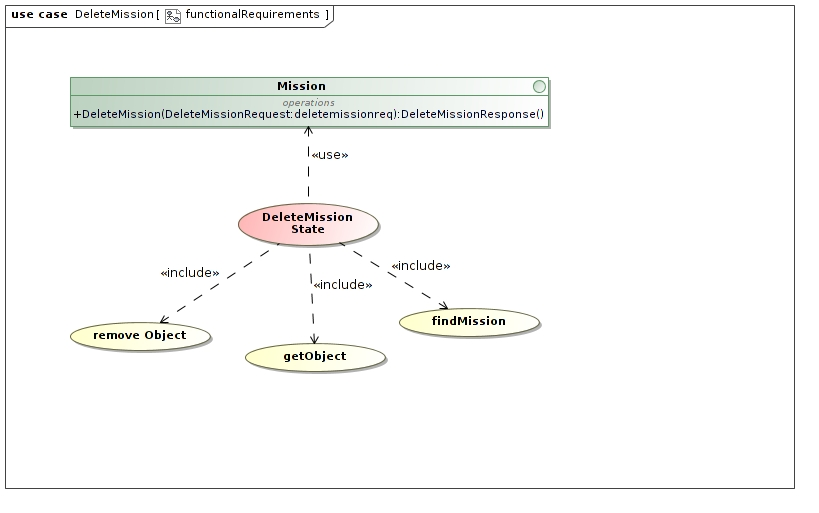
\includegraphics[width=\textwidth]{functionalRequirementsDeleteMission Use Case Diagram.jpg}  \\
					\caption{Use case : deleteMission}
				\end{figure}
				
				\begin{figure}[H]
					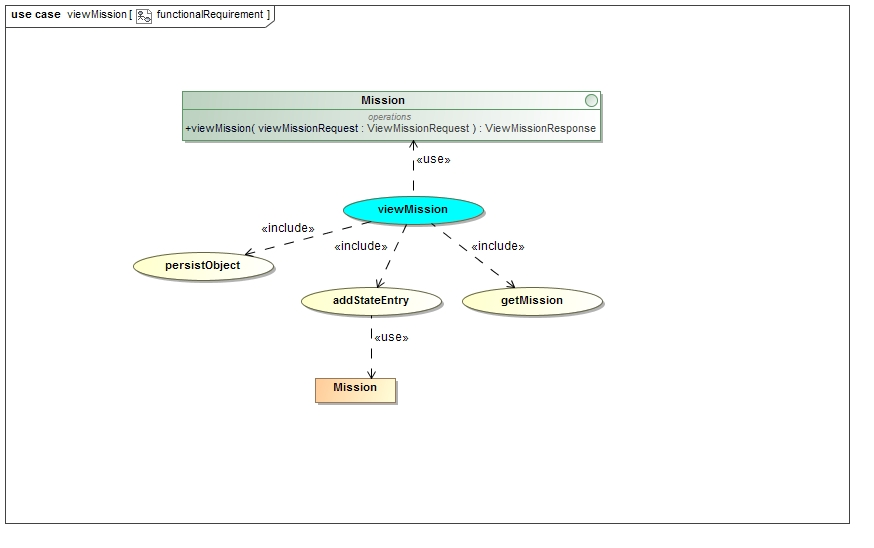
\includegraphics[width=\textwidth]{functionalRequirement_viewmission.jpg}  \\
					\caption{Use case : viewMission}
				\end{figure}

			\textbf{Nice-To-Have}
				\begin{itemize}
	  				\item Edit mission
				\end{itemize}
				
				\begin{figure}[H]
					\includegraphics[width=\textwidth]{functionalRequirementsEditmissin Use case Diagram.jpg}  \\
					\caption{Use case : viewMission}
				\end{figure}
		\end{flushleft}
\end{document}
